\scanpage{56}
% archive foliation: 55
% lines 1-8
\begin{tabular}{c}
U N I V E R S I T E\\
DES SCIENCES ET TECHNIQUES\\
DU LANGUEDOC\\
\texttt{------------}\\
Service de la Scolarité\\
MR/GJ\\
Diffusion : Liste H\\
N° 3758
\end{tabular}

MONTPELLIER, le 15 Juin 1978
% line 9
\uline{AVIS DE SOUTENANCE D'UNE THESE DE DOCTORAT D'ETAT}
% line 10
\uline{Nom et prénom du candidat} : WALTER Philippe
% lines 11-12
\uline{Titre de la thèse} : Recherches écologiques et biologiques sur les Scarabéides Co-\\
prophages d'une savane du Zaïre.
% lines 13-14
\uline{Date, heure et lieu de soutenance prévus} : 3 JUILLET 1978 à 9 Heures 30 mn

Salle de cours n° 6, U.S.T.L.
% line 15
\uline{Nom du Directeur de thèse} : Monsieur le Professeur Renaud PAULIAN.
% line 16
\uline{Désignation du laboratoire où la thèse est préparée} : Zoologie (Professeur LEGENDRE)
% lines 17-24
\uline{Résumé de la thèse} : Les recherches ont été effectuées sur le Plateau Bateke zaïrois.

Les résultats sont présentés en trois parties :

1) le peuplement (composition d'ensemble, aspects biogéographiques, répartition dans les différentes formations végétales, fluctuations des densités de population, sex-ratio)

2) observations autoécologiques et biologiques (préférences trophiques, heures d'activité, éthologie)

3) morphologie larvaire : description détaillée de 12 larves.
% line 25
\uline{Durée approximative des recherches ayant abouti à la thèse} : 5 ans 1/2.
% lines 26-29
\uline{Noms des Rapporteurs} :

\begin{tabular}{ll}
PAULIAN R. & , Professeur, Zoogéographie, Rectorat BORDEAUX\\
LAMOTTE M. & , Professeur, Ecologie, Ecole Normale Supérieure PARIS\\
LEGENDRE R. & , Professeur, Zoologie Ecologie, U.S.T.L.
\end{tabular}
% lines 30-40
\uline{Composition du jury} :

\begin{tabular}{lp{.75\linewidth}}
LEGENDRE R. & , Professeur, Zoologie Ecologie, U.S.T.L.\\
& (Président)\\[1ex]
PAULIAN R. & , Professeur, Zoogéographie, Rectorat BORDEAUX\\
LAMOTTE M. & , Professeur, Ecologie, Ecole Normale Supérieure PARIS\\
& (Membres extérieurs choisis en raison de leur compétence scientifique)\\[1ex]
EUZET L. & , Professeur, Parasitologie, U.S.T.L.\\
& (Membre étranger à la spécialité du candidat)\\
LUMARET J.-P. & , Maître-assistant, Biogéographie, Univ. MONTPELLIER III.\\
BARAUD J. & ., Professeur, Biochimie, Univ. BORDEAUX
\end{tabular}
% lines 41-43
Le Secrétaire Général,

\figure{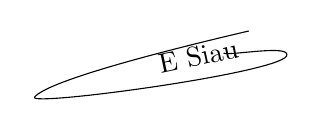
\begin{tikzpicture}[scale=.8]
\node[rotate=12] at (.5,.2) {\unsure{E Siau}};
\draw (1.3,.6) .. controls (-.2,.25) and (-1.9,-.2) .. (-2.1,-.45) .. controls (-2.2,-.6) and (1.7,-.08) .. (1.9,.2) .. controls (2,.4) and (1,.2) .. (.9,.25);
\end{tikzpicture}}

\uline{E. SIAU}
